We decided to have time tracking data stored in Git Notes for every repo so that it can be tightly tied to code.
This gives us opportunity to have more complete overview when and on what issue / branch the time was spent.
It also gives access to a features such as git diff that can be used for measuring writing speed.
Furthermore, it lifts a job from our shoulders by handling complex cases such as rebase and merge for us.

The downside is that git notes take up some space on client machine and Git server.
They can also be externally edited, and they might cause issues with git usage if developer does not follow best practices.
Nonetheless, we decided to go this way as the space used by git notes is fractional compared to file sizes, and our app is a tool for the developer,
so we don't see any urgent need to protect it from him.

We also found open source CLI app made for local time-tracking with Git, so we decided to base our app on the already existing code and add more functionality.
There is always an option to switch to external database for storing this kind of data but there is no reason to so at the moment.

Partly enforced by the usage of git, the general design is shown on Figure
\ref{fig:project-archidecture}.

\begin{figure}[h]
    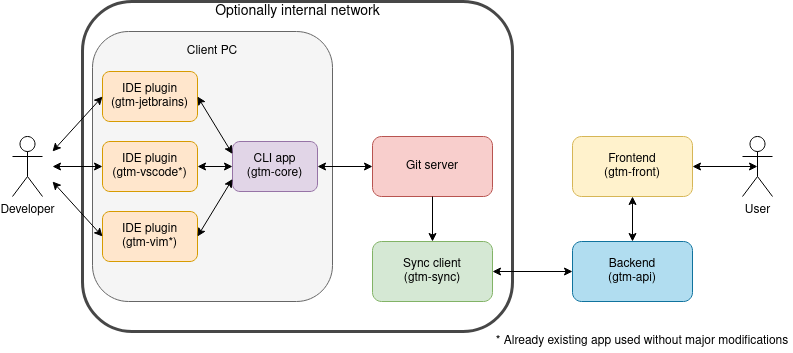
\includegraphics[width=\textwidth]{figures/project_archidecture}
    \caption{Application general design}
    \label{fig:project-archidecture}
\end{figure}

The general time-tracking application can be divided into three different kind of smaller applications:
\begin{enumerate}
    \item \textbf{Applications that are responsible for data collecting.} These applications are CLI app and IDE plugins and are installed on developers machine.
    \item \textbf{Applications that are responsible for syncing data.} This role is filled by a Sync client, and these applications are installed onto companies servers where they can access git internal network.
    \item \textbf{Applications that are responsible for analyzing and displaying data.} These are Frontend and Backend app that can be installed on any public server.
\end{enumerate}

The reasoning behind this architecture is scalability and security.
For every Backend there can be multiple Sync clients all installed on different machines and with different Git access rights.
For every Sync client there can be multiple Client apps all logging time independent of one another.
And in the end, there can be multiple IDE plugins interacting with CLI app.

For security, it is very important to ensure, that no sensitive information is leaked.
To deal with this issue many companies have their Git available only in an internal network.
Not to rise any more security concerns we decided to follow the same principle and not export any git code outside internal network.
That is the reason, why Sync client is needed as it has access to internal network, but only uploads time-tracking related information to our Backend.
Therefore, actual code never leaves an internal network.

All the applications that are installed on either client machine or client server are open source so that the client can easily verify,
they only do what they are meant to do.

To properly manage numerous apps in different programming languages we decided to have each app source code in separate git repository.
This reduces the amount of merge conflicts and also makes building CI/CD easier.

\section{Client CLI app}\label{sec:cli-app}
%TODO(Tavo): We should somewhere state what are gtm-core, gtm-api, gtm-*
This is the main app on client machine.
The app is responsible for storing events sent by an editor to files and then later also combining the stored information into Git Note.
You can also see all main stats, such as time spent on a commit via CLI app.

The app is based on open source time tracking app \href{https://github.com/git-time-metric/gtm}{Git-Time-Metric} written in Go and licenced under MIT licence.
We decided to base our app on Git-Time-Metric solution because their app was working the way we wanted to, it had plenty of users meaning plenty of testing done,
and the Git-Time-Metric app had good code style.

Although the app was already working we still needed to do many bug fixes and add some features it didn't have.
The biggest change in design was that we removed copied in dependencies to git submodules.
Although this seems like a small step it turned out to be very complex to build go linked with C library dynamically.
As we didn't manage to get on dependency to properly work in Windows environments we decided to leave it separately fetched and built in ci/cd workflow file.
Nonetheless, all "snapshot" dependencies were removed.

\section{IDE plugins}\label{sec:ide-plugins}
IDE plugins installed on developer IDE, and they execute CLI app commands on specific editor events.
Plugins are needed to listen for editor events such as typing without having to give CLI app extensive permissions to run in background.
They also provide a simple way to display some information in IDE.
For example time since last commit is show to user inside IDE.

Currently, we only have one plugin that is compatible with all Jetbrains IDE's.
The gtm-jetbrains plugin is written in Kotlin and uploaded to Jetbrains plugin repository so that you can easily install it in your Jetbrains IDE.
Kotlin was chosen as the plugin was limited to JVM based language and only Java and Kotlin were widely supported.
We have experience in both Java and Kotlin, but we both preferred Kotlin to Java due to its null safety and functional patterns.

\section{Sync client}\label{sec:sync-client}
Sync client is run on a network, where it can access git repositories.
On git push, hook sends request to gtm-sync via HTTP request.
Then gtm-sync fetches git repository with its time data, extracts required data and syncs it up to Backend.

The gtm-sync application was written in Rust as it had more up to date library for libgit2 than both Java and Go, required for interacting with git.
Although we did not have prior experience with Rust we preferred it to C/C++ as it is memory safe and it has higher level libraries that can be
used for building a web server and API client.
Python and NodeJS were ruled out because they produce very big memory footprint compared to Rust, and they also run a lot slower.
Neither of them also gives a type safety.

For the code design, we followed domain based architecture.
%TODO(Tavo): Folders description?

\section{Backend}\label{sec:backend}
%TODO(Marten): ...

\section{Frontend}\label{sec:frontend}
%TODO(Marten): ...